\documentclass[11pt]{article}
\usepackage{graphicx}


\begin{document}
	
	
	
\begin{enumerate}
	
	%%%%%
	% This item assesses the objectives: 
	% - Evaluating proposed solutions to problems based on appropriateness of methods and accuracy with which these methods are applied
	% - Evaluate solutions to see if they are reasonable and consistent with practical considerations
	%%%%%
	
	\item The population of a small town is given by $P(t) = 2000(1.02)^t$ where $P$ is in people and $t$ is in years since 1980. 
	\begin{enumerate}
		\item Set up -- \emph{but do not evaluate} -- an expression involving limits that would find the instantaneous rate of change in the town's population in the year 2013. 
		\item Suppose we wanted to evaluate the above limit expression using only algebraic operations and no numerical or graphical estimation. Do you think this method of solution would be appropriate for this problem? Explain. 
		\item Here is a graph of $P(t)$ along with the tangent line to the graph of $P$ when $t = 25$. Use these to estimate the instantaneous rate of change in the population of the town in 2005. State your answer clearly and  explain in one sentence how you got your answer. 
		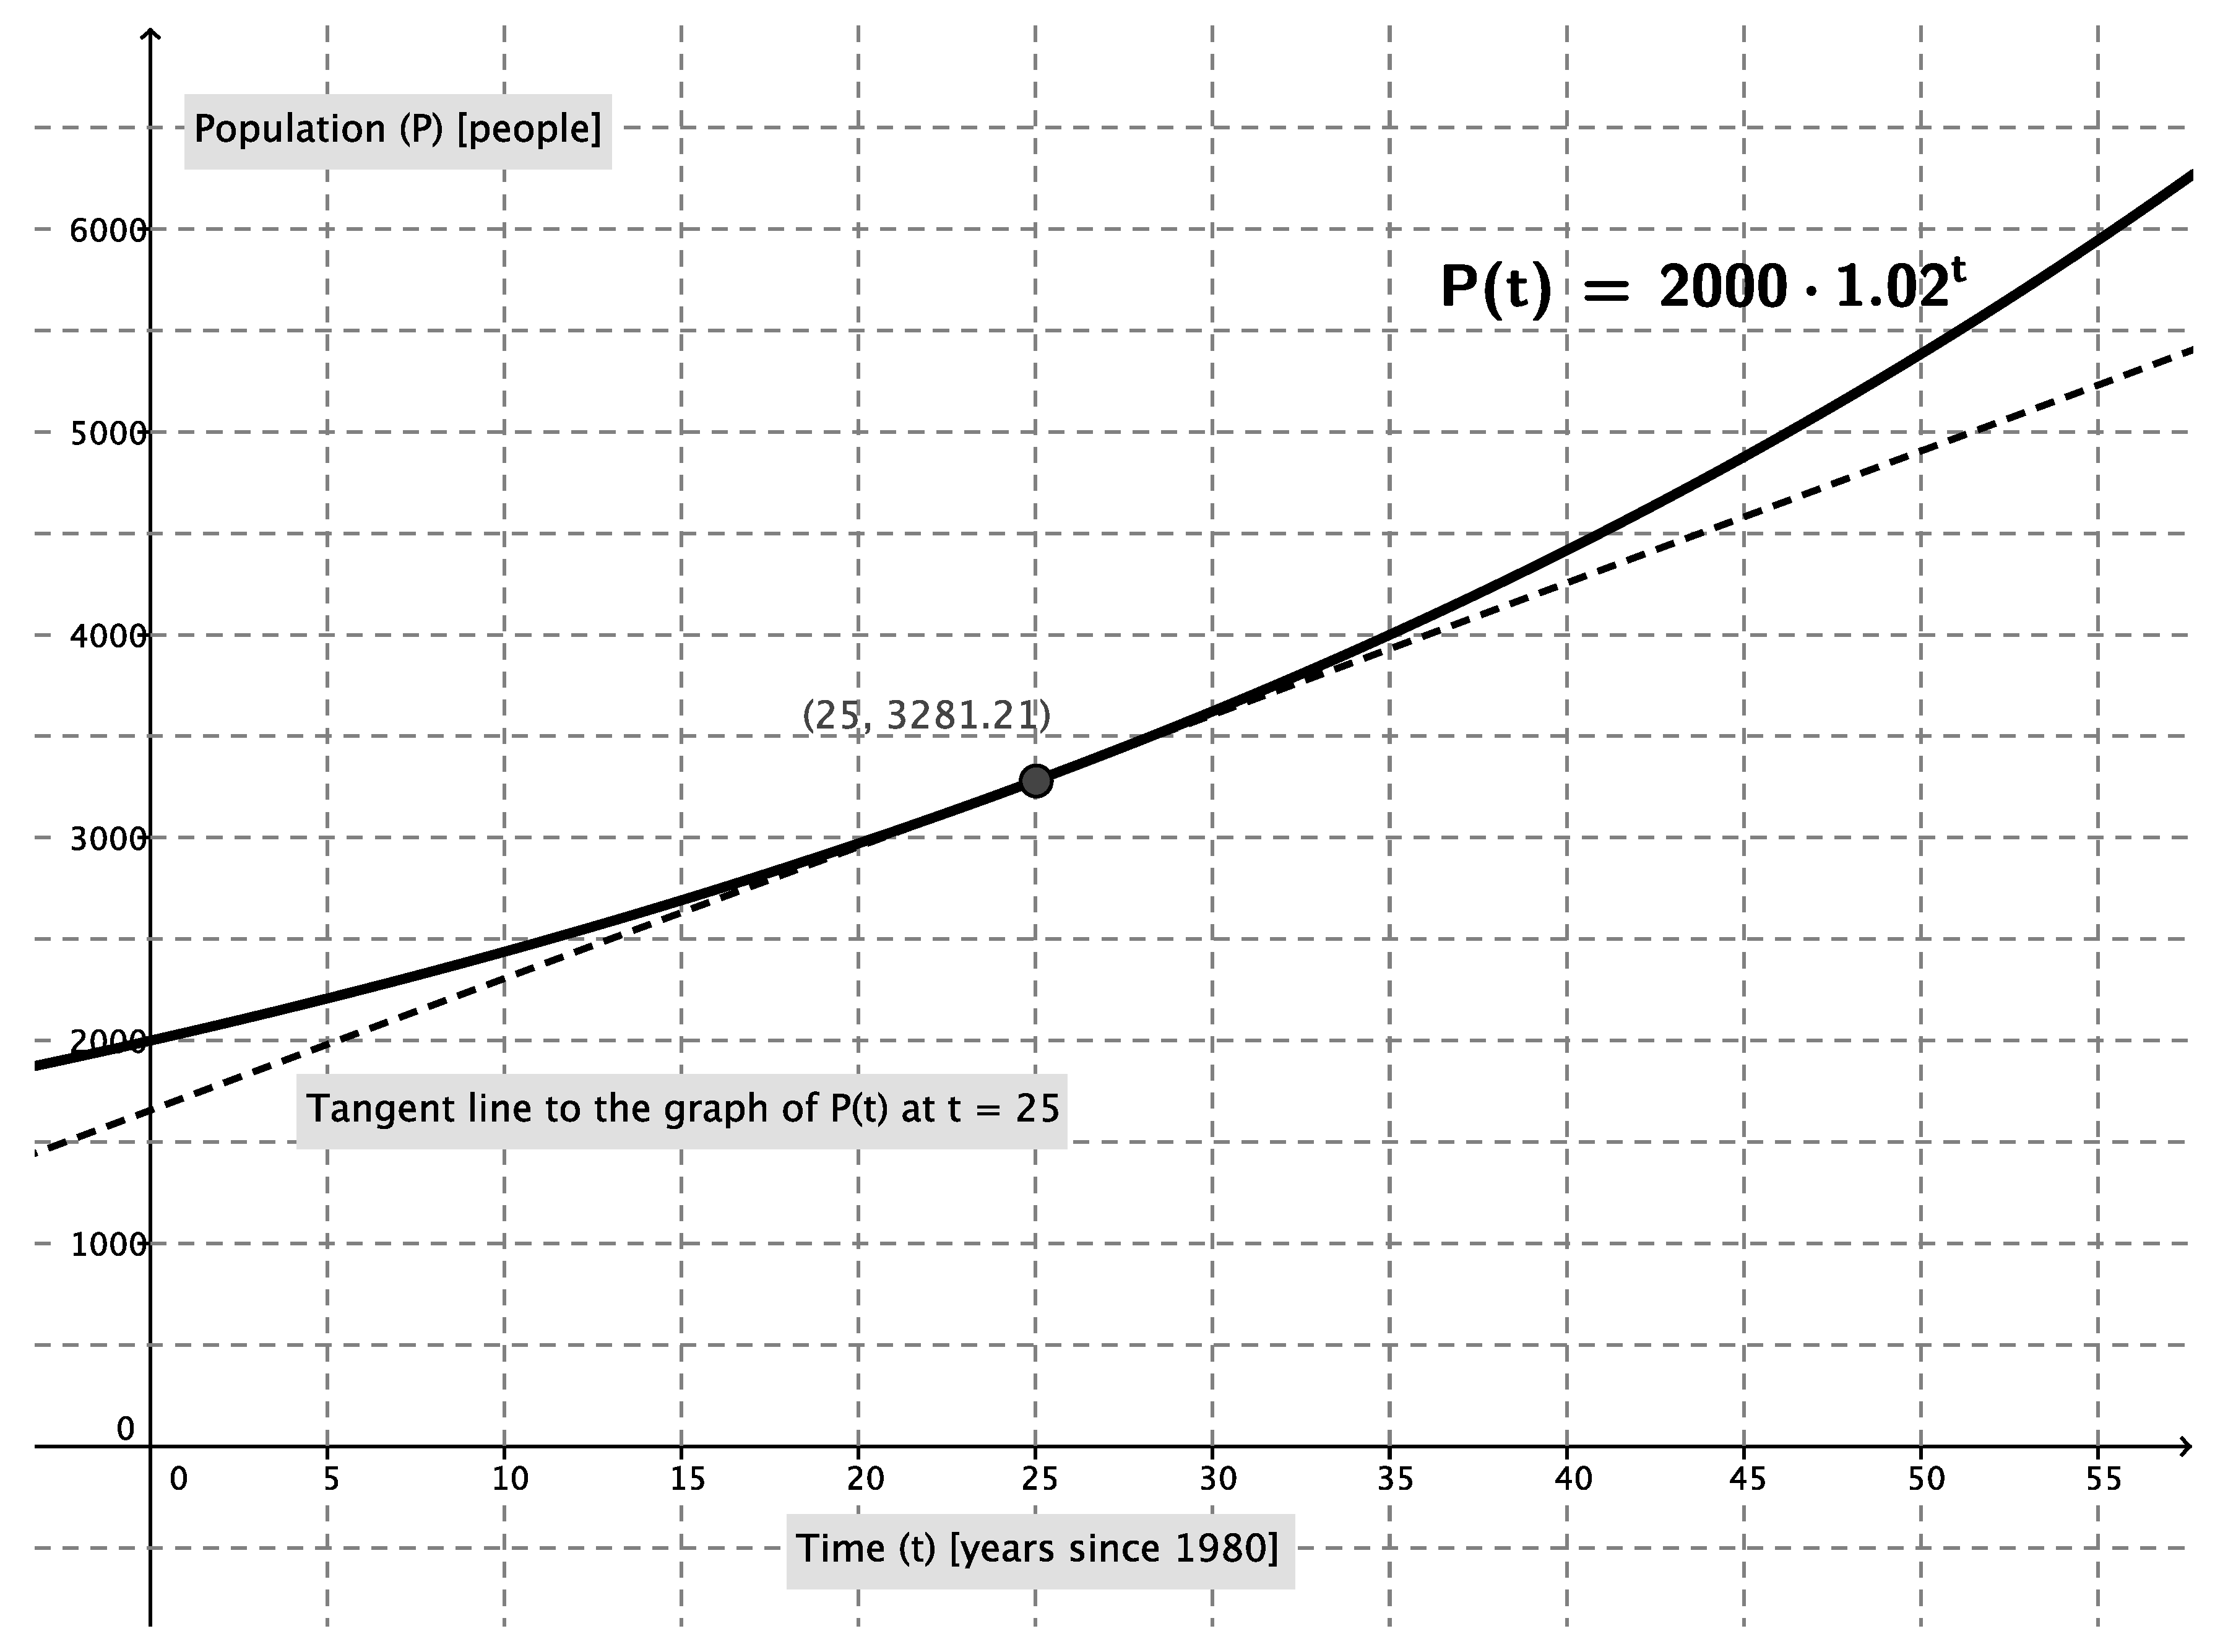
\includegraphics[width=0.6\textwidth]{a1-plot3}
		\item Suppose a student did part (c) of this problem and came up with an answer of $-450$. Is  this solution reasonable and consistent with practical considerations? Explain your reasoning. 
	\end{enumerate}

	%%%%%
	% This item assesses the objectives: 
	% - Algebraic, numerical, graphical techniques to solve problems involving derivatives
	% - Application of derivative to problems involving graphs, numerical data, and equations
	%%%%%

	\item The financial value of a mutual fund goes up and down over time. Suppose that a certain mutual fund's value $V$ (in dollars) is a function of time $t$ (in months since January 2010). In particular note that January 2012 corresponds to the time value $t = 24$, July 2012 is $t=30$, and January 2013 is $t = 36$. Suppose we also know the following information about the value of the mutual fund: 
	\[ V(24) = 8500 \qquad V(30) = 8700 \qquad V(36) = 10300 \qquad V'(36) = 200 \qquad V''(36) = -30 \]
	
	\begin{enumerate}
		\item Find the average rate of change in the value of the mutual fund from January 2012 to July 2012. Show your work and put correct units on your answer. 
		\item Use a central difference to approximate the value of the instantaneous rate of change in the value of the mutual fund in July 2012. Show your work and put correct units on your answer.
		\item Find the local linearization of $V$ when $t=36$, and then use the local linearization to predict the value of the mutual fund in July 2013.
		\item Which is more likely to be greater: The actual value of the mutual fund in July 2013, or the estimated value you calculated in part (c)? Explain your reasoning, and base your reasoning only on the data presented in this problem. 
	\end{enumerate}


\end{enumerate}
	
\end{document}